 \documentclass{beamer}
%
% Choose how your presentation looks.
% For more themes, color themes and font themes, see:
% http://deic.uab.es/~iblanes/beamer_gallery/index_by_theme.html
%
\mode<presentation>
{
  \usetheme{Madrid}      % or try Darmstadt, Madrid, Warsaw, ...
  \usecolortheme{seahorse} % or try albatross, beaver, crane, ...
  \usefonttheme{serif}  % or try serif, structurebold, ...
  \setbeamertemplate{navigation symbols}{}
  \setbeamertemplate{caption}[numbered]
  \setbeamertemplate{itemize/enumerate body begin}{\large}
\setbeamertemplate{itemize/enumerate subbody begin}{\large}
\setbeamertemplate{itemize/enumerate subsubbody begin}{\large}

  \usepackage{amsmath}
  \usepackage{tcolorbox}
  \usepackage[export]{adjustbox}
  \tcbuselibrary{most}
  \usepackage{arydshln}
  \usepackage{tikz}
  \usetikzlibrary{plotmarks}
  \usepackage{pgfplots}
 %\usepackage{enumitem}
%\usepackage{enumerate}
  %\usepackage[shortlabels]{enumitem}
} 


\definecolor{myblue}{RGB}{65,105,225} 
\definecolor{myorange}{RGB}{250,190,0}

\setbeamercolor{structure}{fg=white,bg=myorange}
\setbeamercolor*{palette primary}{fg=myblue,bg=myorange}
\setbeamercolor*{palette secondary}{fg=white,bg=myblue}
\setbeamercolor*{palette tertiary}{bg=myblue,fg=white}
\setbeamercolor*{palette quaternary}{fg=white,bg=myorange!50}

\setbeamercolor{frametitle}{fg=black!90!myblue}

\setbeamercolor{section in head/foot}{fg=white,bg=myblue}
\setbeamercolor{author in head/foot}{fg=black,bg=myorange}
\setbeamercolor{title in head/foot}{fg=white,bg=myblue}

\setbeamertemplate{navigation symbols}{}

\setbeamertemplate{itemize/enumerate body begin}{\large}
\setbeamertemplate{itemize/enumerate subbody begin}{\large}


\defbeamertemplate*{headline}{mytheme}
{%
  \begin{beamercolorbox}[ht=2.25ex,dp=3.75ex]{section in head/foot}
    \insertnavigation{\paperwidth}
  \end{beamercolorbox}%
}%

\defbeamertemplate*{footline}{mytheme}
{
  \leavevmode%
  \hbox{%
  \begin{beamercolorbox}[wd=.5\paperwidth,ht=2.25ex,dp=1ex,right]{author in head/foot}%
    \usebeamerfont{author in head/foot}\insertshortauthor\hspace*{2em}
  \end{beamercolorbox}%
  \begin{beamercolorbox}[wd=.5\paperwidth,ht=2.25ex,dp=1ex,left]{title in head/foot}%
    \usebeamerfont{title in head/foot}\hspace*{2em}\insertshortsubtitle\hspace*{2em}
    \insertframenumber{} / \inserttotalframenumber
  \end{beamercolorbox}}%
  \vskip0pt%
}

\usepackage[english]{babel}
%\usepackage[utf8x]{inputenc}
\usepackage{xcolor}
\usepackage{listings}
\usepackage{pgf}  
\usepackage{textpos}
\usepackage{tabulary}
\usepackage{scrextend}
\usepackage{hyperref}
\usepackage{setspace}
\usepackage{rotating}
\lstset
{
    language=[LaTeX]TeX,
    breaklines=true,
    basicstyle=\tt\scriptsize,
    %commentstyle=\color{green}
    keywordstyle=\color{blue},
    %stringstyle=\color{black}
    identifierstyle=\color{magenta},
}
\newcommand{\bftt}[1]{\textbf{\texttt{#1}}}
%\newcommand{\comment}[1]{{\color[HTML]{008080}\textit{\textbf{\texttt{#1}}}}}
\newcommand{\cmd}[1]{{\color[HTML]{008000}\bftt{#1}}}
\newcommand{\bs}{\char`\\}
\newcommand{\cmdbs}[1]{\cmd{\bs#1}}
\newcommand{\lcb}{\char '173}
\newcommand{\rcb}{\char '175}
\newcommand{\cmdbegin}[1]{\cmdbs{begin\lcb}\bftt{#1}\cmd{\rcb}}
\newcommand{\cmdend}[1]{\cmdbs{end\lcb}\bftt{#1}\cmd{\rcb}}

\newcommand{\wllogo}{\textbf{Overleaf}}

% this is where the example source files are loaded from
% do not include a trailing slash
\newcommand{\fileuri}{https://raw.githubusercontent.com/GiancarloSucci/UniBo.IDSEPC.A2022/main/A2022.IDSEPCLaTeX/}


\usepackage{stackengine}
\def\Ruble{\stackengine{.67ex}{%
  \stackengine{.48ex}{\textsf{P}}{\rule{.8ex}{.12ex}\kern.6ex}{O}{r}{F}{F}{L}%
  }{\rule{.8ex}{.12ex}\kern.6ex}{O}{r}{F}{F}{L}\kern-.1ex}



%----------------------------------------------------------------------------------------
%	TITLE PAGE
%----------------------------------------------------------------------------------------
\title[L04]{Artificial Intelligence, Blockchain, e Criptovalute nello Sviluppo Software \newline\newline
Lezione 6: Distributed Cognition and Extended Mind} % The short title appears at the bottom of every slide, the full title is only on the title page

\author[{\tiny Giancarlo Succi }]{Giancarlo Succi\\\\ Dipartimento di Informatica -- Scienza e Ingegneria\\Universit\`{a} di Bologna\\
\bftt{g.succi@unibo.it}
} % Your name
\institute[unibo] % Your institution as it will appear on the bottom of every slide, may be shorthand to save space


\date{} % Date, can be changed to a custom date

\setbeamertemplate{navigation symbols}{}
\AtBeginSection[]
{
        \begin{frame}<beamer>{Outline}
                \tableofcontents[currentsection]
        \end{frame}
}
\begin{document}

\begin{frame}
\titlepage % Print the title page as the first slide

\end{frame}

%=============================================

\addtobeamertemplate{frametitle}{}{%
\begin{textblock*}{10mm}(-0.01mm,-0.95cm)

\includegraphics[width=0.9cm]{unibo-logo.png}
\end{textblock*}}

%=============================================


\begin{frame}
{\centerline{Structure of the lecture}}
\begin{itemize}
    \item The concept of cognition
    \item Early models
    \begin{itemize}
        \item Attribution theory
        \item The na\"{i}ve scientist
        \item Stereotypes
        \item Heuristics
    \end{itemize} 
    \item Impulsive / Reflective model
    \item Implications for software production
    \item \textcolor{blue}{Everything we discuss here are \textcolor{red}{\bf working hypotheses}: we have to remember that working hypotheses even if later proved to be wrong, helped the progress of science and technology, e.g., celestial spheres}
\end{itemize} 
\begin{center}
    \tiny{Refer to \url{https://en.wikipedia.org/wiki/Celestial_spheres}}
\end{center}

\end{frame}

\begin{frame}
{\centerline{A working hypothesis}}

\begin{center}

 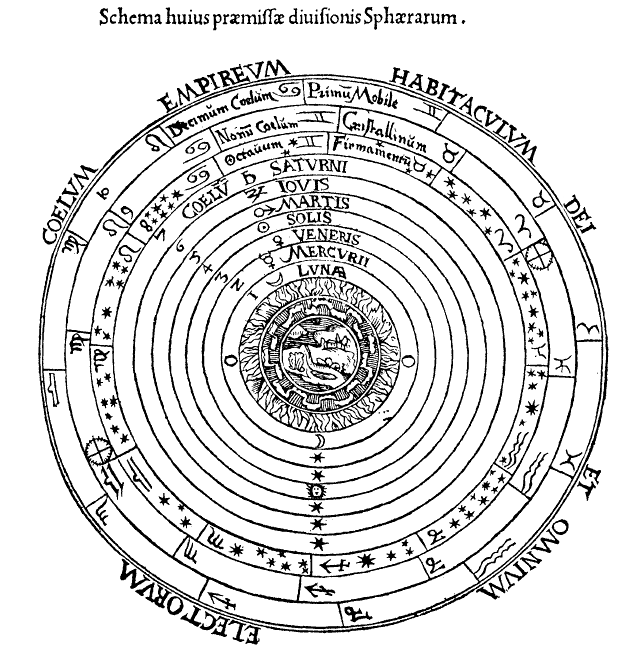
\includegraphics[width=6cm]{P2023.AIBCCSS.KnowledgeAcquisitionRetentionUse/Ptolemaicsystem.png}
 
 \end{center}


\begin{center}
    \tiny{Picture taken from \url{https://en.wikipedia.org/wiki/Celestial_spheres}}
\end{center}
\end{frame}


\begin{frame}
{\centerline{Cognition}}
\begin{itemize}
    \item Our goal in this lecture is to present some paradigms discussing:
    \begin{itemize}
        \item how information is acquired and stored
        \item how such information is then used to make decisions
    \end{itemize}
    \item In this context we review existing models of knowledge throughout their historical evolution
\end{itemize} 
\end{frame}

\begin{frame}
{\centerline{Storing information}}
\begin{itemize}
    \item There have been proposals to divide the storage of information in the human brain in two (or three) parts:
    \begin{itemize}
        \item short term memory
        \item long term memory
        \item (working memory)
    \end{itemize}
    \item we will now shortly review such concepts
\end{itemize} 
\end{frame}


\begin{frame}
{\centerline{General Model}}

\begin{center}

 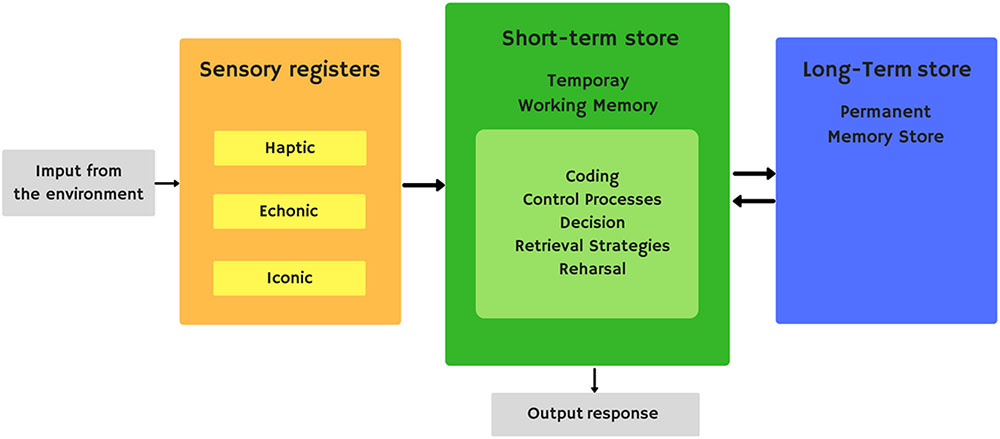
\includegraphics[width=12cm]{P2023.AIBCCSS.KnowledgeAcquisitionRetentionUse/MemoryStructure.jpg}
 
 \end{center}


\begin{center}
    \tiny{Picture taken from 
    Camina Eduardo, G\"{u}ell Francisco (2017). ``The Neuroanatomical, Neurophysiological and Psychological Basis of Memory: Current Models and Their Origins.'' Frontiers in Pharmacology 8}
\end{center}

\end{frame}

\begin{frame}
{\centerline{Short Term Memory}}
\begin{itemize}
    \item Short term memory is a function of the brain finalized of storing information ready to be used for a short amount of time
  \item The time-span for storage of such information is of the order of 18 seconds
  \item Repetition helps in increasing the time the information is stored there
  \item Capacity is believed to be of 7 $\pm$ 2 elements
  \item Some researchers include in it the working memory
\end{itemize} 

\begin{center}
    \tiny{Taken from \url{https://en.wikipedia.org/wiki/Short-term_memory}\\
    Camina Eduardo, G\"{u}ell Francisco (2017). ``The Neuroanatomical, Neurophysiological and Psychological Basis of Memory: Current Models and Their Origins.'' Frontiers in Pharmacology 8}
\end{center}

\end{frame}

\begin{frame}
{\centerline{Long Term Memory}}
\begin{itemize}
    \item Long term memory is where the information is kept for a indefinite amount of time
  \item It is further divided into:
  \begin{itemize}
  \item explicit (declarative) memory, then further divided into:
  \begin{itemize}
  \item   episodic memory
  \item semantic memory
  \item (autobiographic memory)
  \end{itemize} 
  \item implicit (non declarative) memory, then further divided into:
    \begin{itemize}
  \item   procedural memory
  \item emotional memory
  \end{itemize} 
\end{itemize} 
\end{itemize} 


\begin{center}
    \tiny{Taken from \url{https://en.wikipedia.org/wiki/Long-term_memory}}
\end{center}

\end{frame}

\begin{frame}
{\centerline{Typical Schema of Long Term Memory}}

\begin{center}

 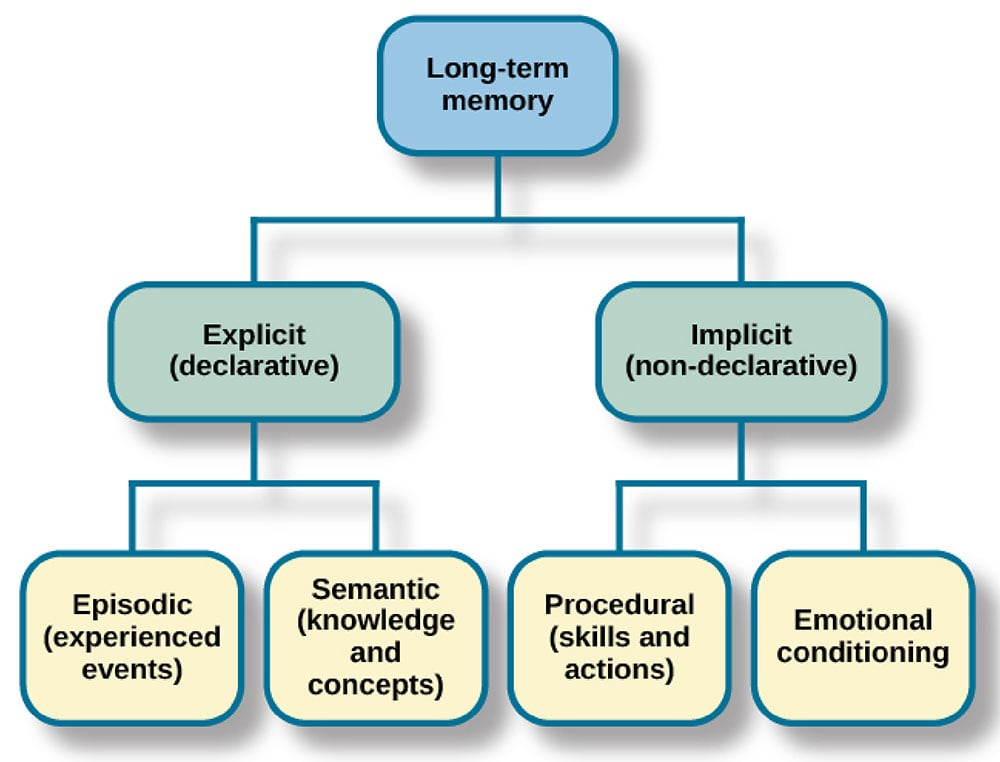
\includegraphics[width=8cm]{P2023.AIBCCSS.KnowledgeAcquisitionRetentionUse/LongTermMemory.jpg}
 
 \end{center}


\begin{center}
    \tiny{Image copied from \url{https://simplypsychology.org/long-term-memory.html} visited on 20230304, claimed author there: Saul Mcleod}
    \end{center}

\end{frame}


\begin{frame}
{\centerline{Working Memory (1/2)}}
\begin{itemize}
    \item There are hypotheses that separated from the short term memory there is a memory retaining information for the specific purpose of making computations
    \item Such memory is called working memory
    \item There are proposals suggesting that it is multicomponent
\end{itemize} 

\begin{center}

 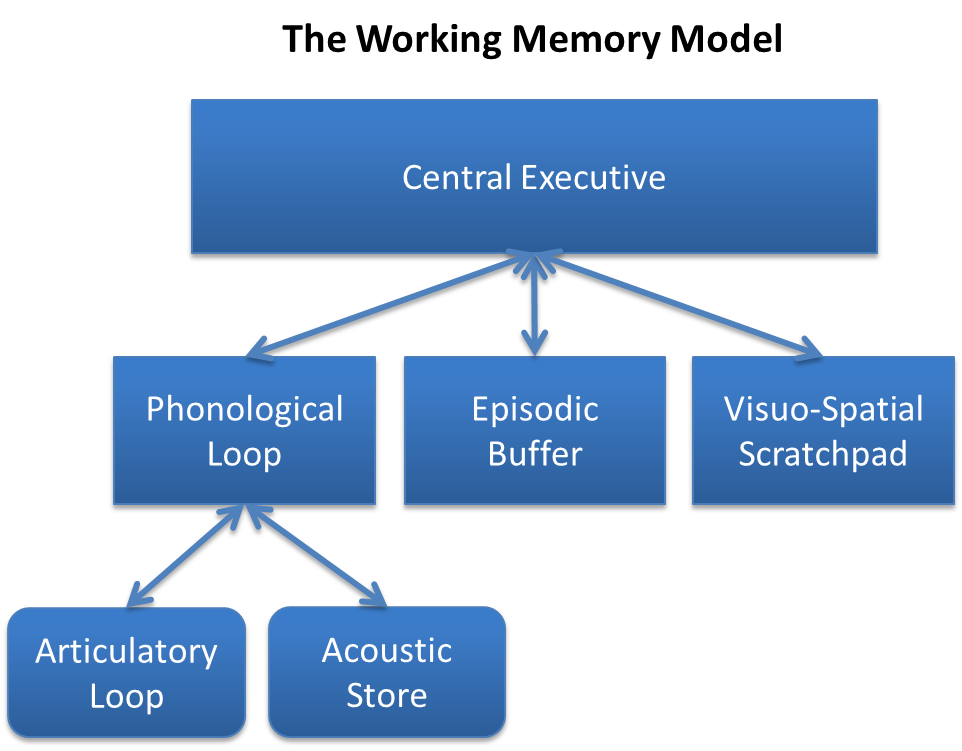
\includegraphics[width=4cm]{P2023.AIBCCSS.KnowledgeAcquisitionRetentionUse/MulticomponentWorkingMemory.png}
 
 \end{center}

\begin{center}
    \tiny{Taken from \url{https://en.wikipedia.org/wiki/Working_memory}. The picture is credited there to come from Baddeley AD, Hitch G (1974). Bower GH (ed.). ``Working Memory. Psychology of Learning and Motivation.'' Vol. 2. Academic Press. pp. 47–89. }
\end{center}

\end{frame}

\begin{frame}
{\centerline{Working Memory (2/2)}}
\begin{itemize}
    \item There are also hypotheses that the working memory is part of the long term memory
    \item Information is extracted from there with a kind of cashing mechanism
\end{itemize} 

\begin{center}

 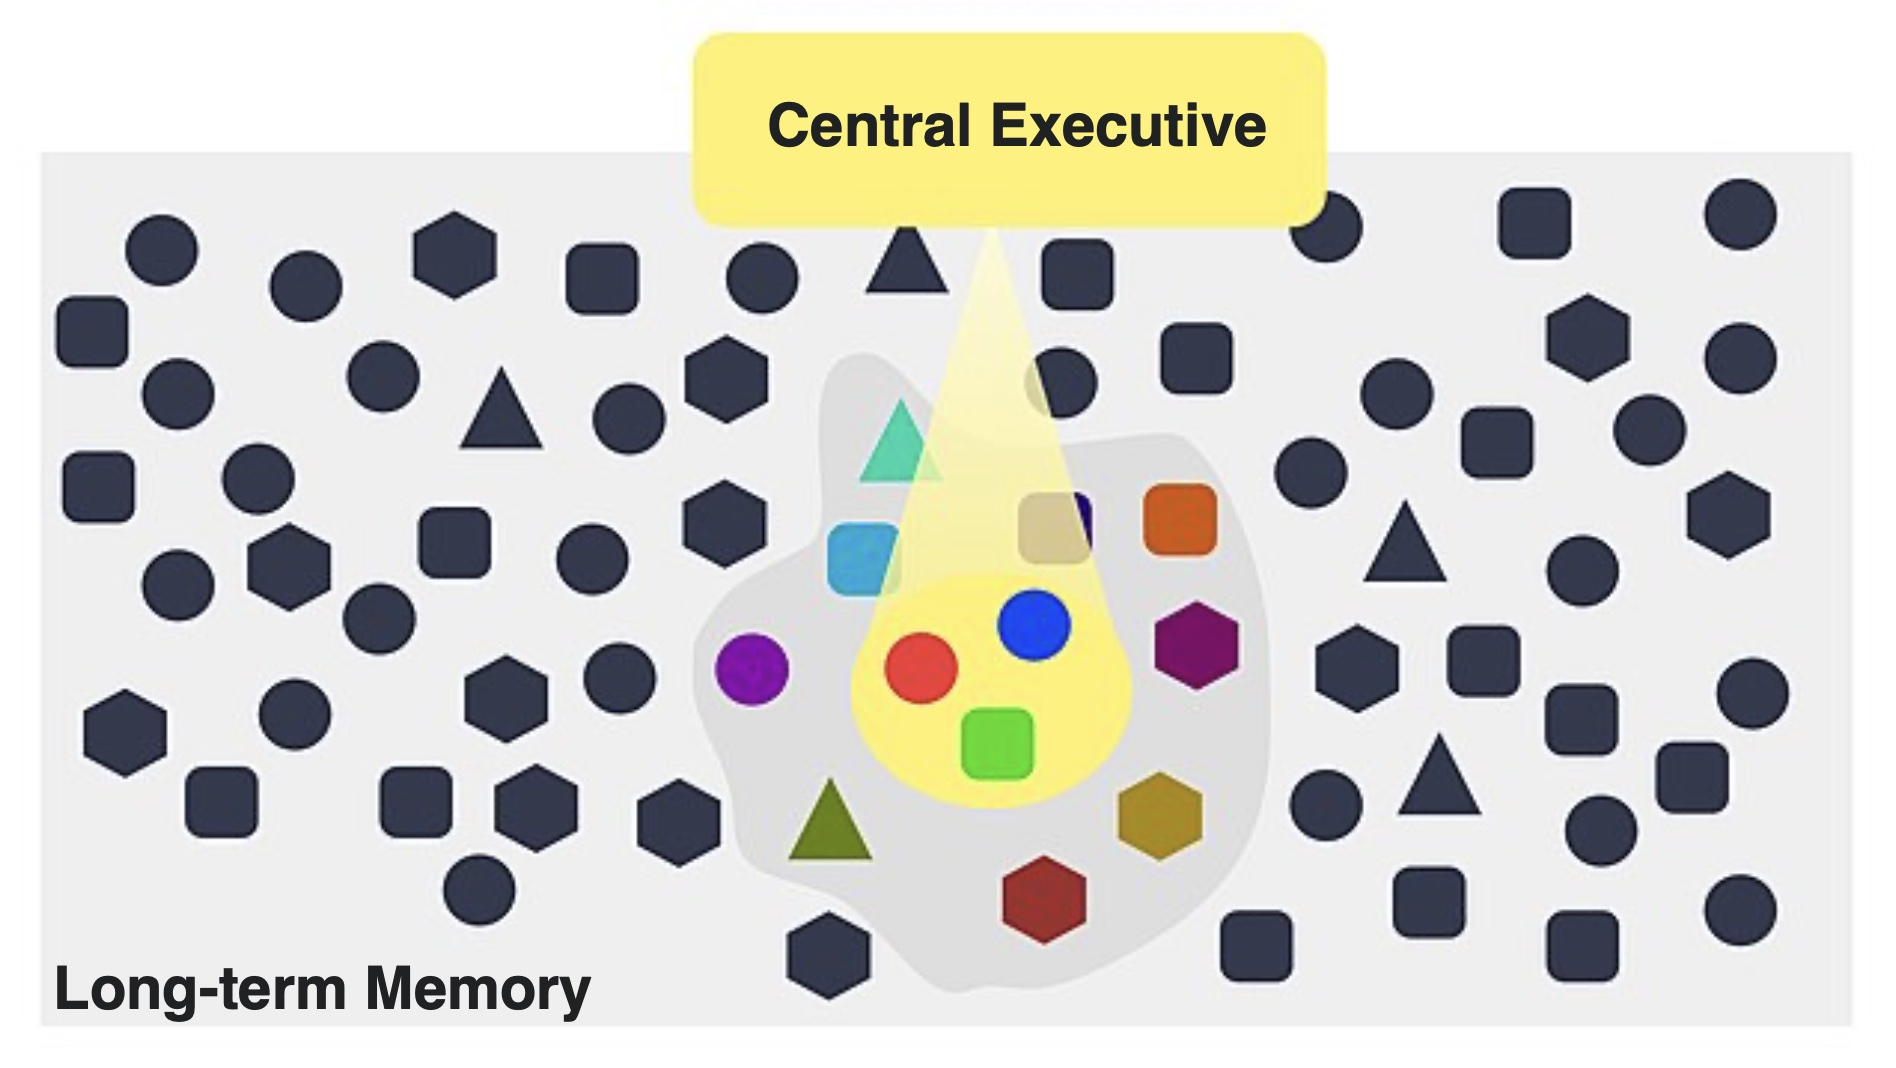
\includegraphics[width=8cm]{P2023.AIBCCSS.KnowledgeAcquisitionRetentionUse/WorkingMemoryPartOfLongTermMemory.jpg}
 
 \end{center}

\begin{center}
    \tiny{Taken from \url{https://en.wikipedia.org/wiki/Working_memory}. The picture is credited there to come from Ericsson KA, Kintsch W (April 1995). ``Long-term working memory.'' Psychological Review. 102 (2): 211–245. }
\end{center}

\end{frame}



\begin{frame}
{\centerline{Using knowledge}}
\begin{itemize}
    \item We now review a series of models of know the knowledge is used to performs actions
    \item We focus on
    \begin{itemize}
        \item attribution theory and the na\"{i}ve scientist
        \item the cognitive miser 
        \item the motivated tactician
        \item the impulsive / reflective model
    \end{itemize}
    \item considering a historical evolution
\end{itemize} 
\end{frame}

\begin{frame}
{\centerline{Attribution theory (1/2)}}
\begin{itemize}
    \item How do individuals attribute properties to entities they perceive?
    \item How do individuals attribute causes for what happens around them?
    \item Attribution bias/error
    \item Locus of causality
    \begin{itemize}
    \item Internal attribution
    \begin{itemize}
    \item attribution of the cause to self
    \end{itemize}
    \item External attribution
    \begin{itemize}
    \item attribution of the cause to the environment
    \end{itemize}
    \end{itemize} 
\end{itemize} 

\begin{center}
    \tiny{Taken from \url{https://en.wikipedia.org/wiki/Attribution_(psychology)}\\
    Heider, F (1944). ``Social perception and phenomenal causality.'' Psychological Review. 51 (6): 358–374.}
\end{center}
\end{frame}

\begin{frame}
{\centerline{Attribution theory (2/2)}}
\begin{itemize}
    \item Typical biases:
    \begin{itemize}
    \item internal attribution:
    \begin{itemize}
        \item positive own situations 
        \item negative situations of others
    \end{itemize} 
    \item external attribution
    \begin{itemize}
        \item negative own situations 
        \item positive situations of others
    \end{itemize} 
    \end{itemize} 
    \item Self-determination and feeling of autonomy
\end{itemize} 

\begin{center}
    \tiny{Taken from \url{https://en.wikipedia.org/wiki/Attribution_(psychology)}\\
    Heider, F (1944). ``Social perception and phenomenal causality.'' Psychological Review. 51(6):358–374.}
\end{center}
\end{frame}

\begin{frame}
{\centerline{The Na\"{i}ve Scientist}}
\begin{itemize}
    \item Humans tries to provide a simple and rational explanation of all the details of the world around them
    \item They use the information available to them that they try to compose like in a puzzle
    \item When doing so they perform attributions
\end{itemize} 
\begin{center}
    \tiny{Taken from \url{https://en.wikipedia.org/wiki/Cognitive_miser}\\
    Duane T. Wegener and Richard E. Petty (1998) ``The naive scientist revisited: Naive theories and social judgment'' Social Cognition. 16(1):1}
\end{center}

\end{frame}

\begin{frame}
{\centerline{Stereotypes}}
\begin{itemize}
    \item Humans are not always able to handle complexity
    \item Understanding complexity requires effort
    \item A stereotype is a reconstruction of the reality where complex details are simplified
    \item Stereotypes are reinforced by looking a facts that from a simplistic perspective correspond to such stereotype
    \item Stereotypes simplify the thinking process
\end{itemize} 
\begin{center}
    \tiny{Taken from \url{https://en.wikipedia.org/wiki/Cognitive_miser}}
\end{center}

\end{frame}

\begin{frame}
{\centerline{Heuristics (1/4)}}
\begin{itemize}
    \item Heuristics are another approach to cope with complexity
    \item We can define them as:
    \begin{itemize}
        \item a fast answer to 
        \item a problem requiring for its full solution a \textcolor{cyan}{complex} procedure
        \item answer that might be \textcolor{red}{occasionally \textbf{wrong}}
   \end{itemize} 
   \item People rely in heuristics to save time and effort
\end{itemize} 
\begin{center}
    \tiny{Taken from \url{https://en.wikipedia.org/wiki/Cognitive_miser}\\
    Kahneman, Daniel and Tversky, Amos (1973) ``On the psychology of prediction.'' Psychological Review. 80 (4): 237–251}
\end{center}

\end{frame}



\begin{frame}
{\centerline{Heuristics (2/4)}}

\begin{itemize}
    \item There are multiple kinds of heuristics:
    \begin{itemize}
        \item \textcolor{red}{representativeness} heuristics:
             \begin{itemize}
                       \item people tend to generalize distributions ignoring the real rules of statistics.
             \end{itemize} 
         \end{itemize} 
\end{itemize} 

       \begin{quote}
 \scriptsize
 A cab was involved in a hit and run accident at night. Two cab companies, the Green and the Blue, operate in the city. 85\% of the cabs in the city are Green and 15\% are Blue.  A witness identified the cab as Blue. The court tested the reliability of the witness under the same circumstances that existed on the night of the accident and concluded that the witness correctly identified each one of the two colours 80\% of the time and failed 20\% of the time. What is the probability that the cab involved in the accident was Blue rather than Green knowing that this witness identified it as Blue? 
 
 {\normalfont \scriptsize (Tversky and Kahneman (1982) as quoted in wikipedia)}

       \end{quote}
\begin{center}
    \tiny{Taken from \url{https://en.wikipedia.org/wiki/Representativeness_heuristic} \\
  Gilovich, T., \& Savitsky, K. (2002). Like goes with like: The role of representativeness in erroneous and pseudo-scientific beliefs. In T. Gilovich, D. Griffin, \& D. Kahneman (Eds.), Heuristics and biases: The psychology of intuitive judgment (pp. 617–624). Cambridge University Press.\\
  Tversky, A., \& Kahneman, D. (1982). Evidential impact of base rates. In D. Kahneman, P. Slovic, \& A. Tversky (Eds.), Judgment under Uncertainty: Heuristics and Biases. Cambridge University Press}
\end{center}

\end{frame}

\begin{frame}
{\centerline{Heuristics (3/4)}}
\begin{itemize}
    \item There are multiple kinds of heuristics:
                 \begin{itemize}
        \item \textcolor{red}{availability} heuristic:
             \begin{itemize}
                       \item ``if something can be recalled, it must be important'' (wikipedia)
                       \item people build their beliefs on facts that come to their mind faster -- typically most recent facts
                       \item people make assumption on distributions on entities, events, etc. based on the frequencies of items of them coming to their minds
             \end{itemize} 
   \end{itemize} 
\end{itemize} 
\begin{center}
    \tiny{Taken from \url{https://en.wikipedia.org/wiki/Availability_heuristic} \\
    Kahneman, Daniel and Tversky, Amos (1973) ``On the psychology of prediction.'' Psychological Review. 80 (4): 237–251}
\end{center}

\end{frame}


\begin{frame}
{\centerline{Heuristics (4/4)}}
\begin{itemize}
    \item There are multiple kinds of heuristics:
                 \begin{itemize}
        \item \textcolor{red}{anchoring} or \textcolor{red}{adjustment} heuristic:
             \begin{itemize}
                       \item people based their opinion on a reference impression (the anchor) and then readjust it based on new information
                       \item often the reference impression is the first impression (but sometimes also the last)
                       \item can be effective in requirement negotiation
             \end{itemize} 
   \end{itemize} 
\end{itemize} 
\begin{center}
    \tiny{Taken from \url{https://en.wikipedia.org/wiki/Anchoring_(cognitive_bias)} \\Kahneman, Daniel and Tversky, Amos (1974) ``Judgment under Uncertainty: Heuristics and Biases.'' Science. 185 (4157): 1124-1131\\
    Yasseri, T., Reher, J. (2022) ``Fooled by facts: quantifying anchoring bias through a large‐scale experiment.'' Journal of Computational Social Science. 5: 1001–1021}
\end{center}

\end{frame}



\begin{frame}
{\centerline{The Cognitive Miser}}
\begin{itemize}
    \item The theory of cognitive miser clusters observations and theories about how people reason on facts
    \item It includes the concepts of stereotypes and heuristics
    \item It is centered on the idea that people tend to be miser (scrooge) in using their cognitive resources when analysing facts and buidling knowledge
    \item The essence is that people make decisions trying to minimize their effort
\end{itemize} 
\begin{center}
    \tiny{Taken from \url{https://en.wikipedia.org/wiki/Cognitive_miser}}
\end{center}

\end{frame}

\begin{frame}
{\centerline{The Motivated Tactician and the Meaning Seeker}}
\begin{itemize}
    \item We can perceive the na\"{i}ve scientist and the cognitive miser as two extremes of a continuous of positions on how the mind works
   \item It has been also proposed that there are also people who may select which option to follow based on the context in which they are
   \begin{itemize}
   \item this gives raise to the concept of \textcolor{red}{\bf motivated tactician}
   \end{itemize} 
   \item there is also the proposal rooted on the concept of Kant categories that are used to represent knowledge as a kind of point in a space of multiple dimensions (the categories)
   \begin{itemize}
   \item the concept of the \textcolor{cyan}{\bf meaning seeker} consider people in the quest for a comprehensive understanding of the work
\end{itemize} 
\end{itemize} 
\begin{center}
    \tiny{Taken from \url{https://en.wikipedia.org/wiki/Cognitive_miser}}
\end{center}

\end{frame}

\begin{frame}
{\centerline{The Motivated Tactician and the Meaning Seeker}}
\begin{itemize}
    \item We can perceive the na\"{i}ve scientist and the cognitive miser as two extremes of a continuous of positions on how the mind works
   \item It has been also proposed that there are also people who may select which option to follow based on the context in which they are
   \begin{itemize}
   \item this gives raise to the concept of \textcolor{red}{\bf motivated tactician}
   \end{itemize} 
   \item there is also the proposal rooted on the concept of Kant categories that are used to represent knowledge as a kind of point in a space of multiple dimensions (the categories)
   \begin{itemize}
   \item the concept of the \textcolor{cyan}{\bf meaning seeker} consider people in the quest for a comprehensive understanding of the work
\end{itemize} 
\end{itemize} 
\begin{center}
    \tiny{Taken from \url{https://en.wikipedia.org/wiki/Cognitive_miser}}
\end{center}

\end{frame}

\begin{frame}
{\centerline{The Dual Process Theory (1/2)}}
\begin{itemize}
    \item Sometimes information is processed and knowledge is created through two different and, sometimes, concurrent processes:
    \begin{itemize}
   \item a \textcolor{red}{conscious}, explicit, and rational (to the extent discussed before) process
   \item an \textcolor{red}{unconscious}, implicit / automatic process
       \begin{itemize}
   \item think for instance at when \textcolor{blue}{we drive the car in ``automatic'' mode} and then we get a high level of attention for something unexpected happening
   \end{itemize} 
      \end{itemize} 
         \item There has been multiple models presenting this duality
   \end{itemize} 
\begin{center}
    \tiny{Taken from \url{https://en.wikipedia.org/wiki/Dual_process_theory}}
\end{center}

\end{frame}

\begin{frame}
{\centerline{The Dual Process Theory (2/2)}}
\begin{itemize}
   \item As an example, Evans suggested that there are:
         \begin{itemize}
   \item an \textcolor{red}{heuristic} process, where the relevant information is selected
   \item an \textcolor{red}{analytical} process, where the information is processed and deductions are made
   \end{itemize}  
   \item There are also theories claiming the opposite:
   \begin{itemize}
   \item the \textcolor{cyan}{dynamic graded continuum} claims that there are a multitude of different possible representations generated by the mind that triggers different reasoning processes depending on situations without assuming a dual process
   \end{itemize}  
   \item particularly interesting is the model of Strack and Deutsch on the \textcolor{blue}{reflective and impulsive dual mode of operations}
   \end{itemize} 
\begin{center}
    \tiny{Taken from \url{https://en.wikipedia.org/wiki/Dual_process_theory}\\Evans, Jonathan (1984). ``Heuristic and analytic processes in reasoning.'' British Journal of Psychology. 75(4):451–468}
\end{center}

\end{frame}

\begin{frame}
{\centerline{The Reflective / Impulsive Model (1/7)}}
\begin{itemize}
\item It explains the reasoning process as the result of two interacting processes:
\begin{itemize}
\item an implicit \textcolor{red}{impulsive} process that reacts fast based on a kind of associative memory
\item an explicit \textcolor{red}{reflective} process that generates knowledge following a reasoning process
   \end{itemize} 
\item the two systems work concurrently, sometimes with coherent results, sometimes in opposition
\item this approach provides an explanation of several phenomena involving the human mind, including, for instance, how software inspections often work 
   \end{itemize} 
\begin{center}
    \tiny{Taken from Strack F, Deutsch R. ``Reflective and impulsive determinants of social behavior.'' Personality and Social Psychology Review. 2004;8(3):220-47.}
\end{center}

\end{frame}

\begin{frame}
{\centerline{The Reflective / Impulsive Model (2/7)}}
\begin{itemize}
    \item The overall model
\end{itemize} 

\begin{center}

 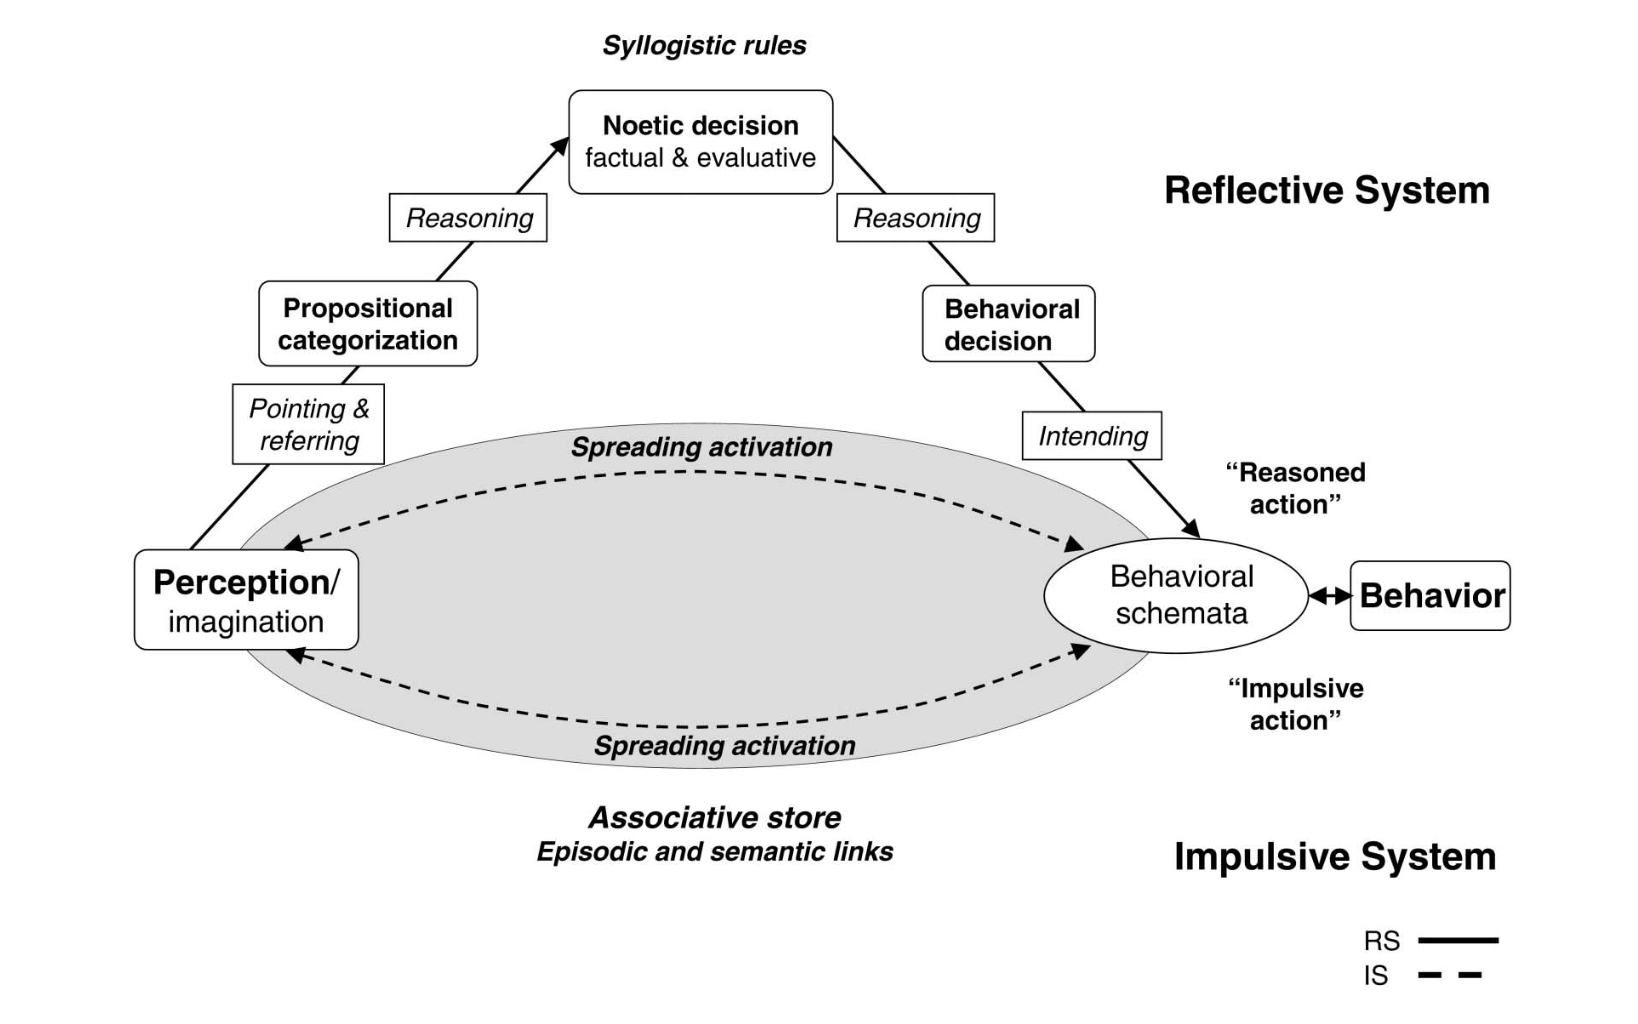
\includegraphics[width=10cm]{P2023.AIBCCSS.KnowledgeAcquisitionRetentionUse/RI.HowItWorks.jpg}
 
 \end{center}


\begin{center}
    \tiny{Picture copied from page 222 of Strack F, Deutsch R. ``Reflective and impulsive determinants of social behavior.'' Personality and Social Psychology Review. 2004;8(3):220-47.}
    \end{center}

\end{frame}


\begin{frame}
{\centerline{The Reflective / Impulsive Model (3/7)}}
\begin{itemize}
    \item Example of synergistic work -- how the concept of elderly person is generated by the impulsive system
\end{itemize} 

\begin{center}

 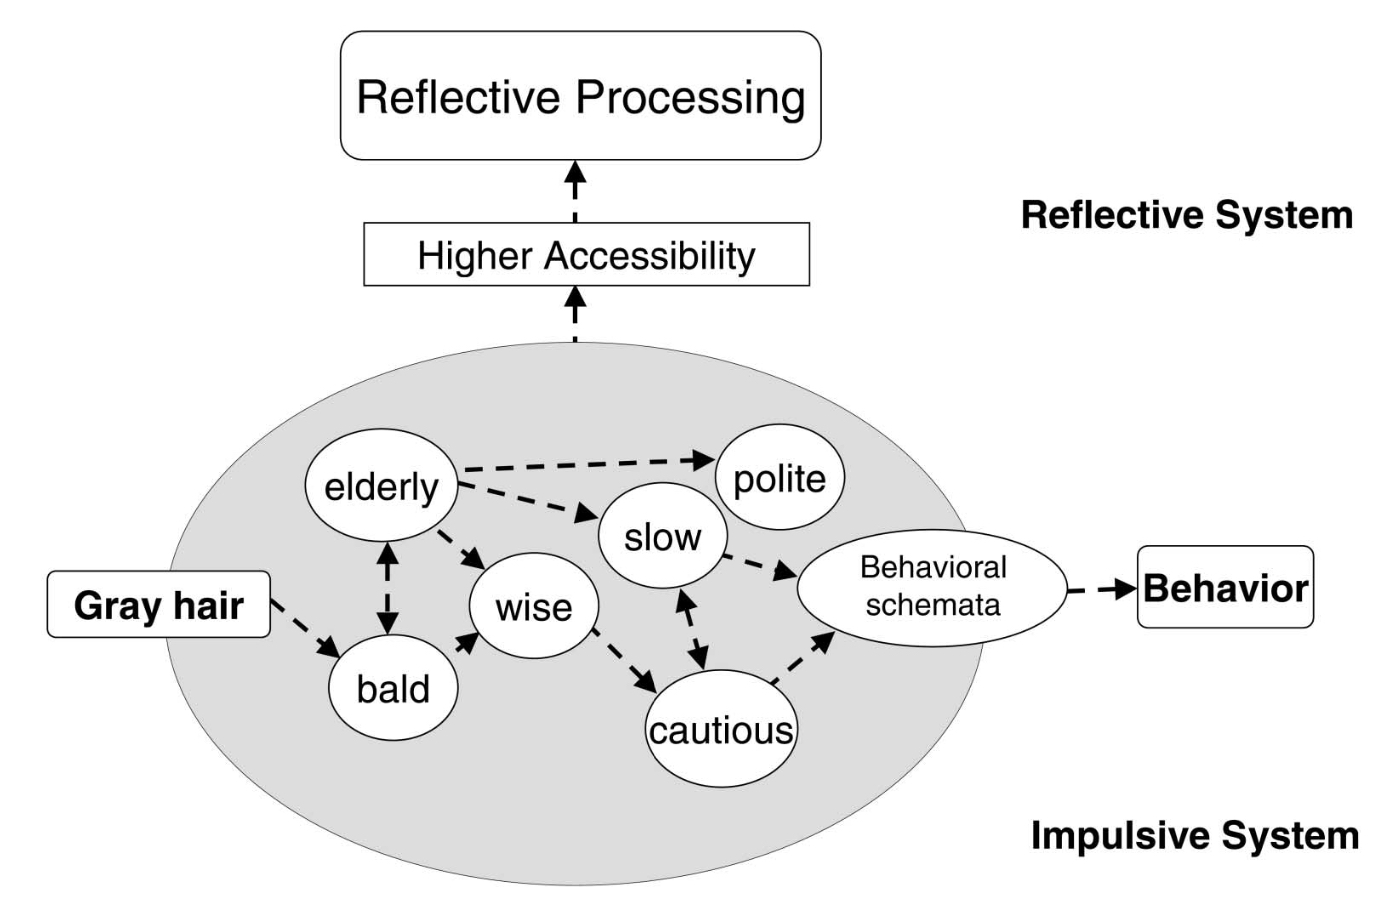
\includegraphics[width=8cm]{P2023.AIBCCSS.KnowledgeAcquisitionRetentionUse/RI.IdentifyingElderly.Impulsive.jpg}
 
\end{center}

\begin{center}
    \tiny{Picture copied from page 224 of Strack F, Deutsch R. ``Reflective and impulsive determinants of social behavior.'' Personality and Social Psychology Review. 2004;8(3):220-47.}
    \end{center}

\end{frame}

\begin{frame}
{\centerline{The Reflective / Impulsive Model (4/7)}}
\begin{itemize}
    \item Example of synergistic work -- how the concept of elderly person is generated by the reflective system
\end{itemize} 

\begin{center}

 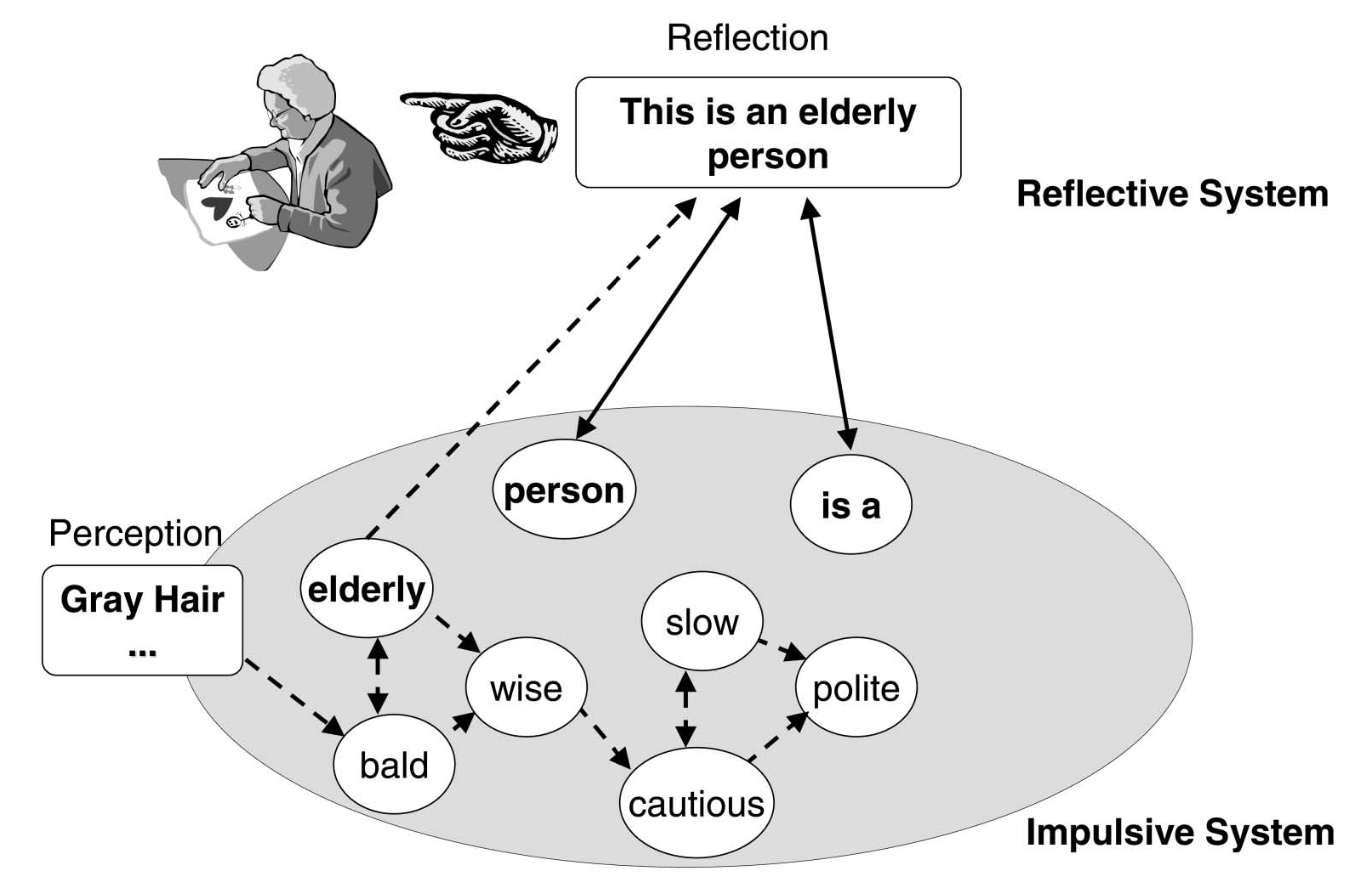
\includegraphics[width=8cm]{P2023.AIBCCSS.KnowledgeAcquisitionRetentionUse/RI.IdentifyingElderly.Reflective.jpg}
 
 \end{center}


\begin{center}
    \tiny{Picture copied from page 225 of Strack F, Deutsch R. ``Reflective and impulsive determinants of social behavior.'' Personality and Social Psychology Review. 2004;8(3):220-47.}
    \end{center}

\end{frame}

\begin{frame}
{\centerline{The Reflective / Impulsive Model (5/7)}}
\begin{itemize}
    \item Example of competing work -- eating the dessert or staying on diet?
\end{itemize} 

\begin{center}

 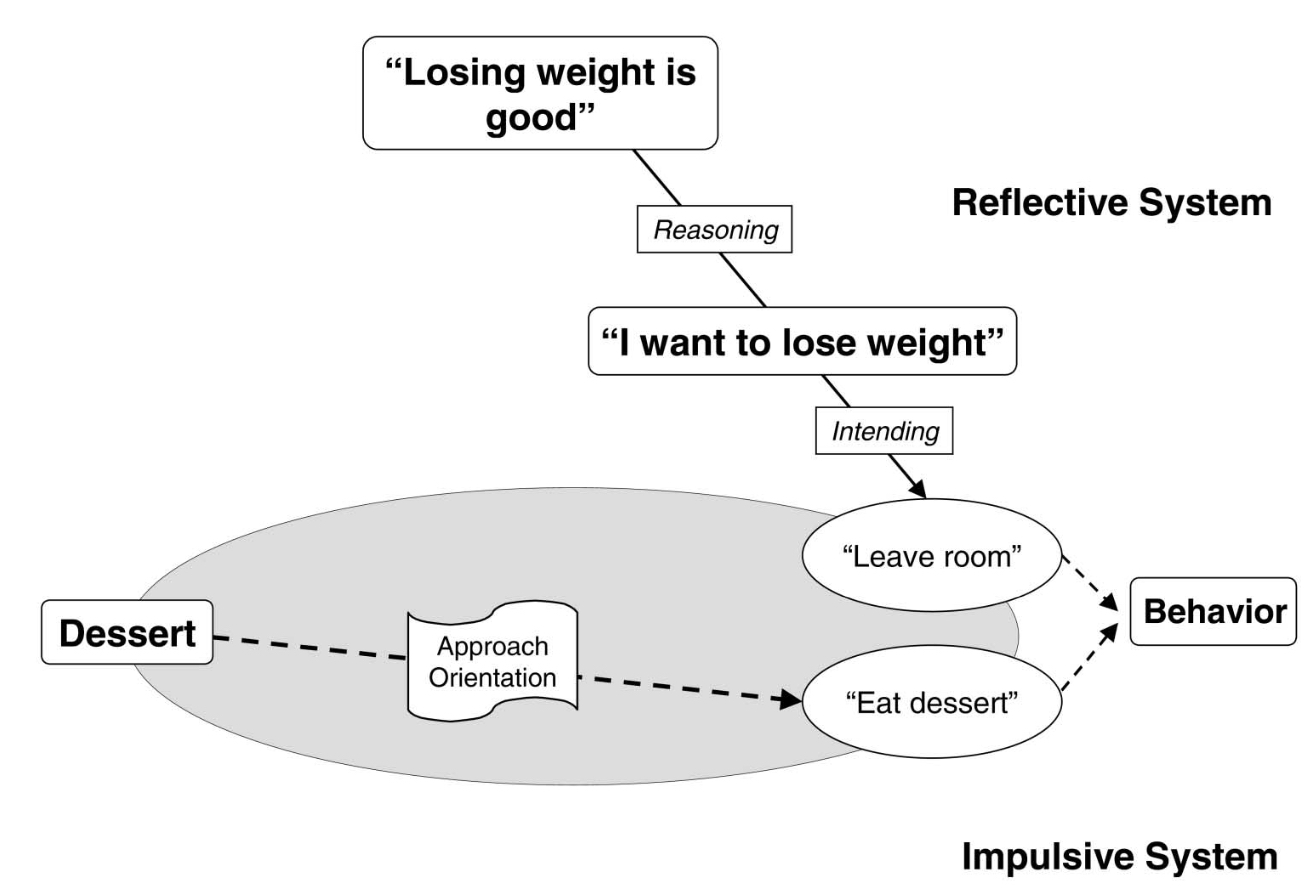
\includegraphics[width=8cm]{P2023.AIBCCSS.KnowledgeAcquisitionRetentionUse/RI.Competing.jpg}
 
 \end{center}


\begin{center}
    \tiny{Picture copied from page 231 of Strack F, Deutsch R. ``Reflective and impulsive determinants of social behavior.'' Personality and Social Psychology Review. 2004;8(3):220-47.}
    \end{center}

\end{frame}

\begin{frame}
{\centerline{The Reflective / Impulsive Model (6/7)}}
\begin{itemize}
    \item How motivational orientation could be explained
\end{itemize} 

\begin{center}

 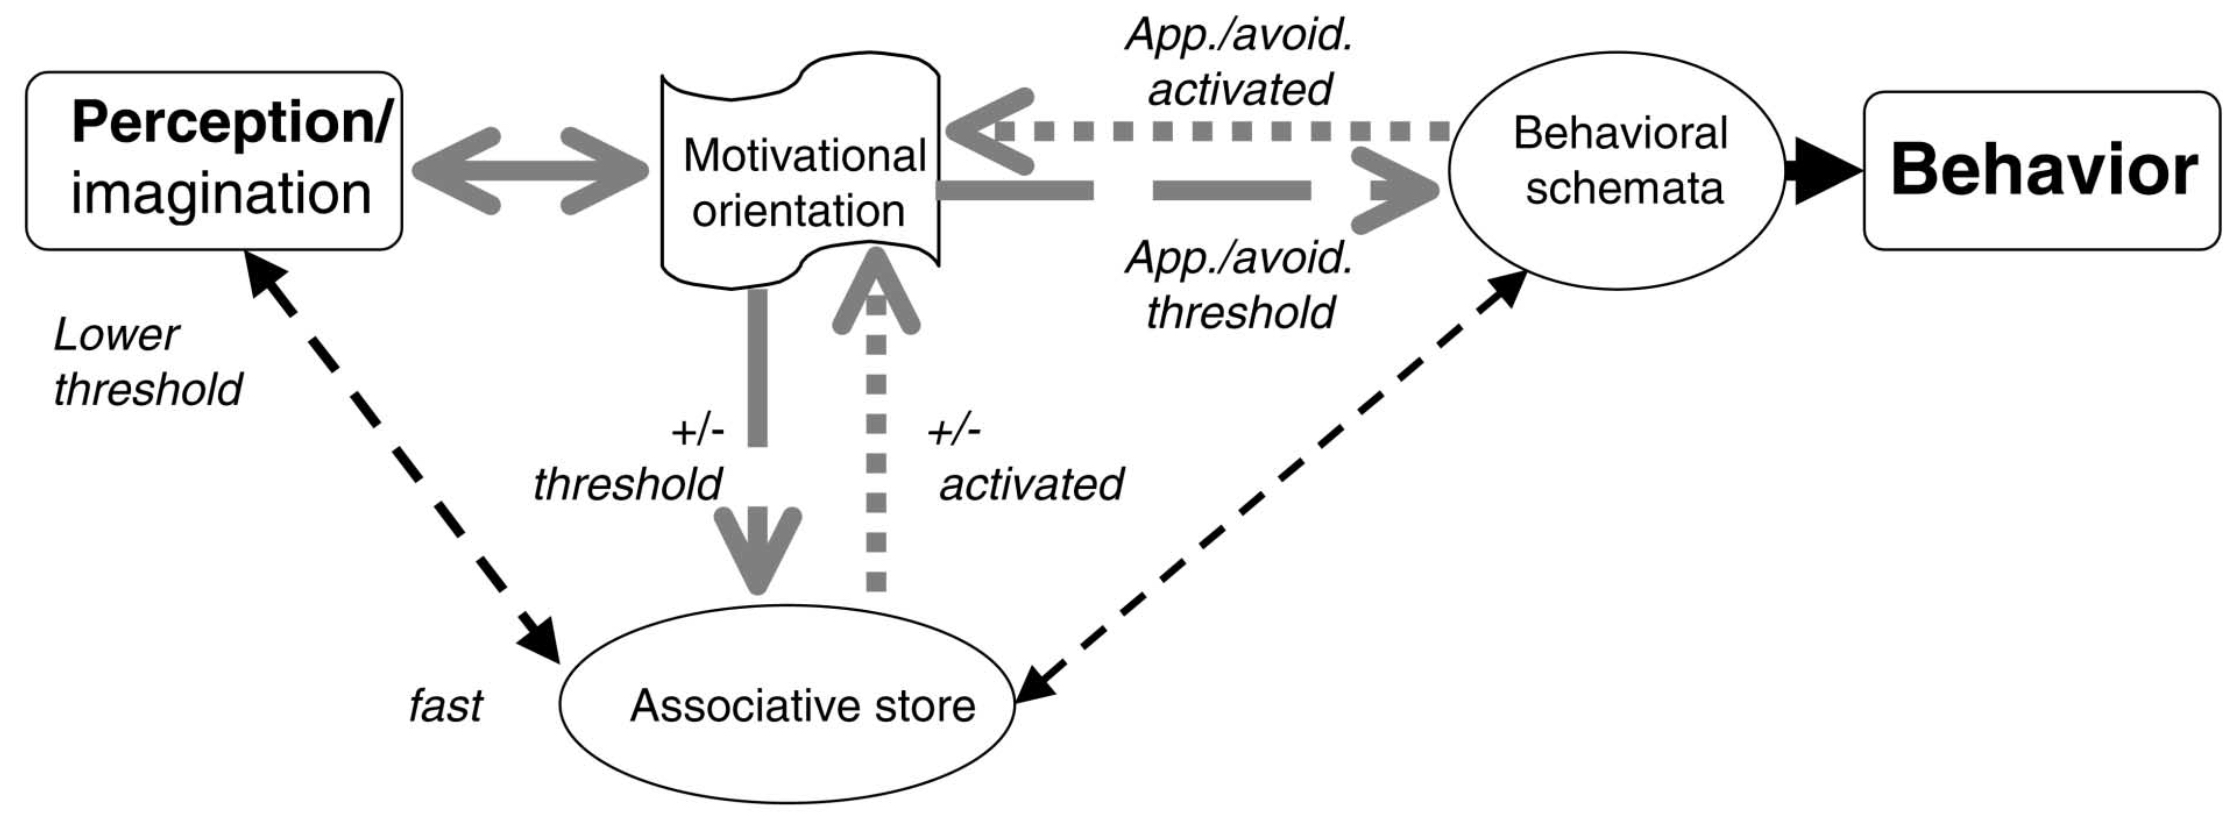
\includegraphics[width=11cm]{P2023.AIBCCSS.KnowledgeAcquisitionRetentionUse/RI.MotivationalOrientation.jpg}
 
 \end{center}

\begin{center}
    \tiny{Picture copied from page 232 of Strack F, Deutsch R. ``Reflective and impulsive determinants of social behavior.'' Personality and Social Psychology Review. 2004;8(3):220-47.}
    \end{center}

\end{frame}


\begin{frame}
{\centerline{The Reflective / Impulsive Model (7/7)}}
\begin{itemize}
    \item Overall view of the model
\end{itemize} 

\begin{center}

 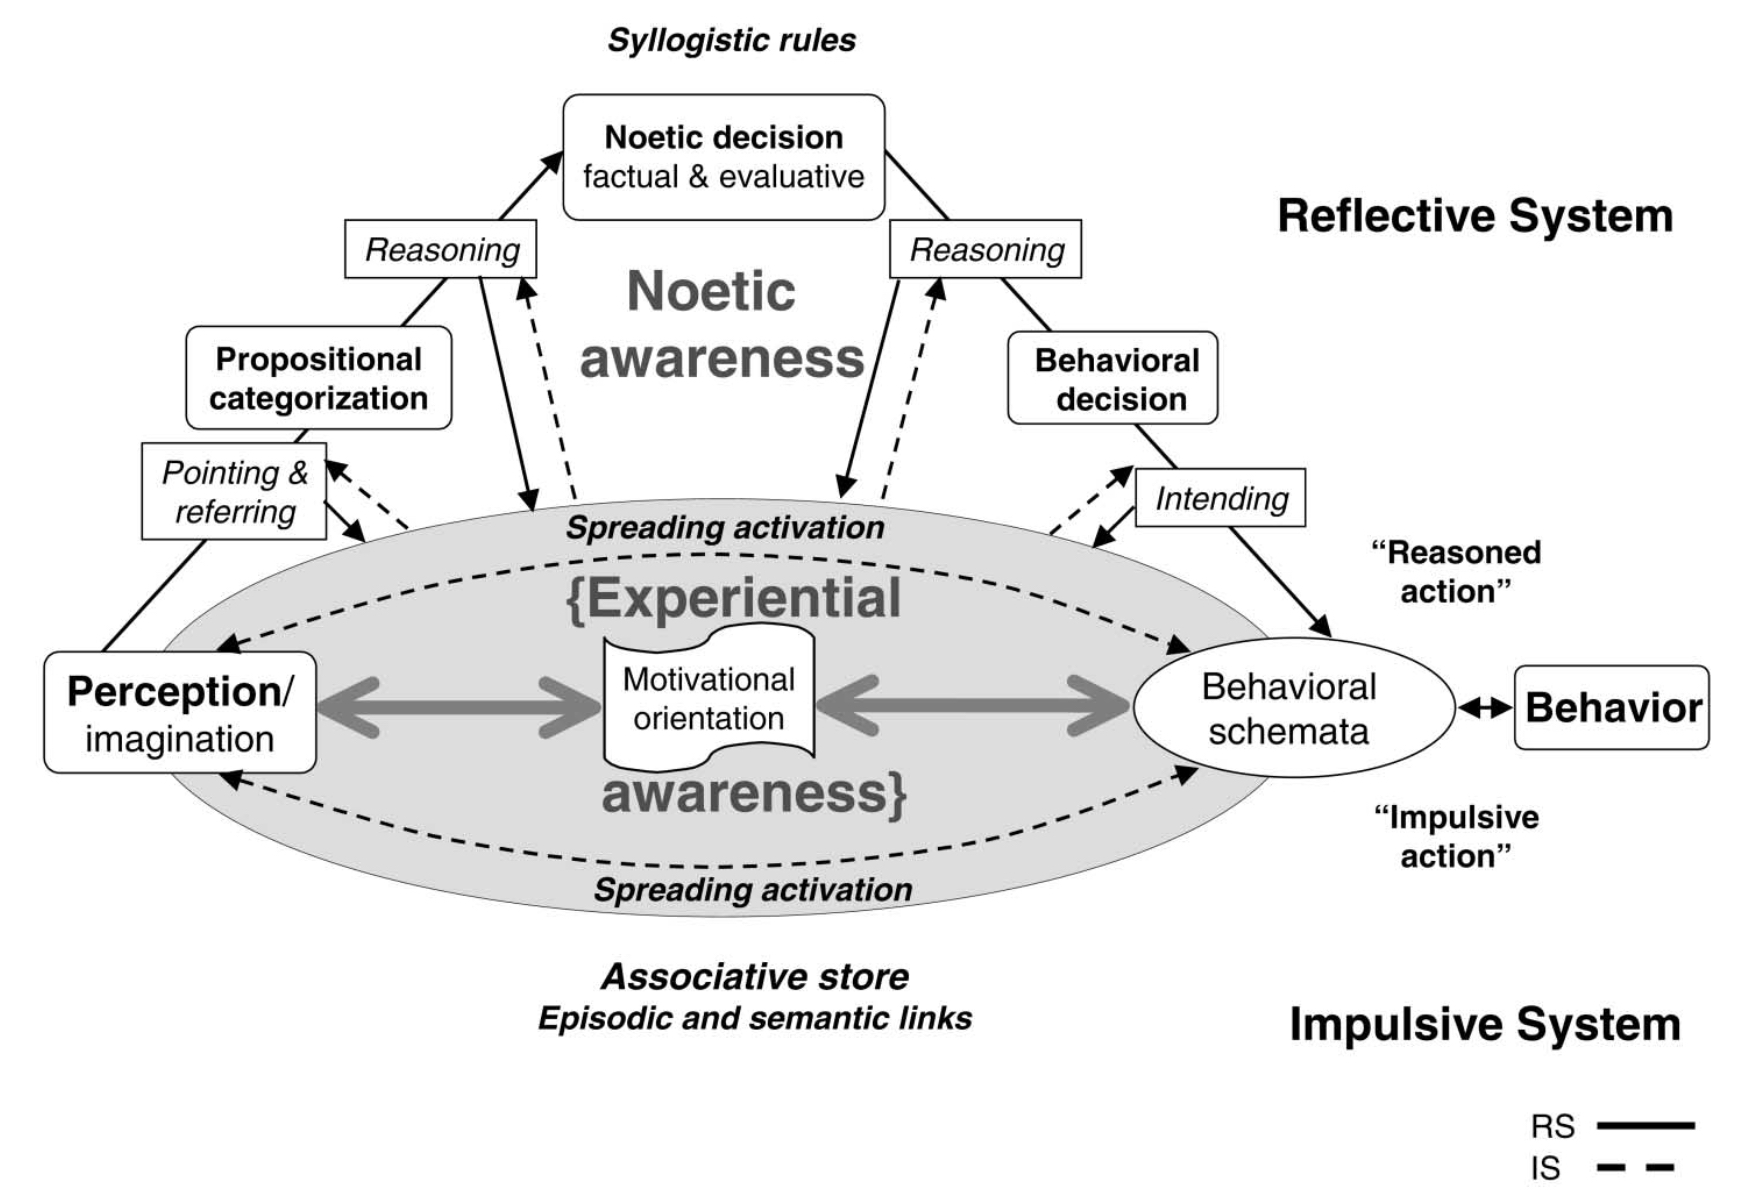
\includegraphics[width=8cm]{P2023.AIBCCSS.KnowledgeAcquisitionRetentionUse/RI.ComprehensiveView.jpg}
 
 \end{center}

\begin{center}
    \tiny{Picture copied from page 239 of Strack F, Deutsch R. ``Reflective and impulsive determinants of social behavior.'' Personality and Social Psychology Review. 2004;8(3):220-47.}
    \end{center}

\end{frame}

\begin{frame}
{\centerline{Questions?}}
\vspace{1cm}
\begin{center}
    \LARGE{End of lecture six.}
\end{center}

\end{frame}


\end{document}
